\section{Modeling a Module}
\SectionPage

\begin{frame}
  \frametitle{How To model A Module?}
  \begin{itemize}
    \item A module needs to:
      \pause
      \begin{itemize}
        \item Initialize some state
        \pause
        \item Update the state based on events
        \pause
        \item Change the view based on the state
      \end{itemize}
      \pause
    \item Module architecture is inspired by Elm and MVC
      \pause
    \item A module should be \textit{pure}
  \end{itemize}
\end{frame}

\hidelogo

\begin{frame}
  \frametitle{Scrapped Architectures}
  \begin{figure}
    \centering
    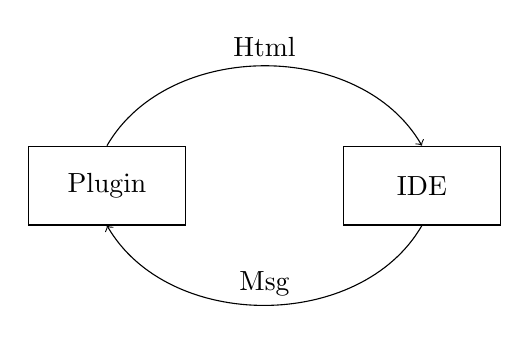
\begin{tikzpicture}
  % Nodes
  \node (p) [rectangle, draw, minimum height=1cm, minimum width=2cm] at (0, 0) {Plugin};
  \node (i) [rectangle, draw, minimum height=1cm, minimum width=2cm] at (4, 0) {IDE};
  % Arrow
  \draw[->] (p.north) to[out=60, in=120] node[midway, above] {Html} (i.north);
  \draw[->] (i.south) to[out=-120, in=-60] node[midway, above] {Msg} (p.south);
  % Header
\end{tikzpicture}


    \caption{Example Module Architecture}
    \label{fig:moduleArchitecture}
  \end{figure}
\end{frame}

\showlogo

\section{Implementation struggles}
\SectionPage

\begin{frame}
  \frametitle{Blasingly Fast Memory Leakage}
  \begin{itemize}
    \item The Rust ABI is not protected by their SemVer notation
      \pause
    \item This means that even a patch to the Rust compiler can break a
      Rust Module
      \pause
    \item Can be fixed by using a Rust Library: \textit{abi\_stable}
      \pause
    \item Had to use `ManuallyDrop` for more complex types, which disables
      the automatic drop
      \pause
    \item Fixed by having Rust modules only reference the state, meaning
      after update and view, the module can be safely dropped
  \end{itemize}
\end{frame}

\begin{frame}
  \frametitle{I Need Super Computer Time For My Featureless App}
  \begin{itemize}
      \pause
    \item JavaScript is more \textit{unsafe} than Rust, due of a lack of typing
      \pause
    \item Need to decode the output from the modules, and catch any exceptions
      \pause
    \item When implementing the init to update to view - cycle, I tested with
      a \textit{basic} module, which should only display "Hello, World!"
      \begin{itemize}
          \pause
        \item The module initialized the state
          \pause
        \item It rendered the view
          \pause
        \item Somehow triggered an update
          \pause
        \item Which triggered a re-render
          \pause
        \item Which triggered an update
          \pause
        \item Which triggered a re-render
          \pause
        \item \dots
      \end{itemize}
  \end{itemize}
\end{frame}

\hidelogo

\begin{frame}
  \frametitle{I Need Super Computer Time For My Featureless App}
  \begin{figure}
    \centering
    \includegraphics[width=0.9\textwidth]{./pics/memory-allocation-zoomed.png}
    \caption{140.6594 Terabytes of memory}
  \end{figure}
\end{frame}

\showlogo
\begin{frame}
  \frametitle{Module V.1 - Final.Final}
  \begin{itemize}
    \item Everything* is a module
      \pause
    \item Modules can \textit{invoke} modules
      \pause
    \begin{itemize}
      \item Init - Returns a set of modifications
    \end{itemize}
    \pause
    \item Pros
    \pause
    \begin{itemize}
      \item Modular
        \pause
      \item Modules can \textit{invoke} other modules
    \end{itemize}
    \pause
    \item Cons
    \begin{itemize}
        \pause
      \item Complex to implement
    \end{itemize}
  \end{itemize}
\end{frame}

\begin{frame}
  \frametitle{Module Type}
  \begin{center}
    \lstinputlisting
    [ language=Haskell
    ]{./code/module-example.hs}
  \end{center}
\end{frame}


\begin{frame}
  \frametitle{Event Type}
  \begin{center}
    \lstinputlisting
    [ language=Haskell
    ]{./code/module-example-event.hs}
  \end{center}
\end{frame}


\begin{frame}
  \frametitle{Counter Example}
  \begin{center}
    \lstinputlisting
    [ language=Haskell
    ]{./code/module-example-counter.hs}
  \end{center}
\end{frame}


\begin{frame}
  \frametitle{Event Handler}
  \begin{center}
    \lstinputlisting
    [ language=Haskell
    ]{./code/module-example-counter-handler.hs}
  \end{center}
\end{frame}
